%| report template for CSUS Senior Design
%|
%| language: LaTeX
%| Author: Ben Smith
%| 
%| This source has been tagged with the "#CHANGE" tag in areas
%| that require updating when making a new docuent
%|
%| This source will generate a PDF file complete with thumbnails navigation menu and metadata,
%| 

\documentclass[12pt,article]{IEEEtran}

%| This section will essentially create variables to be used in some
%| of the documents formatting and the PDF's metadata 
%|
%| 
\newcommand{\TITLE}{Problem Statement}
\newcommand{\KEYWORDS}{}
\newcommand{\ABSTRACT}{The average person is becoming less active, not just in first world countries, 
					but across geopolitical and socioeconomic boundaries. This sedentary lifestyle has 
					dire consequences to health and wellness. Moderate exercise can lead to improved 
					health across all age groups.  We analyze the consequences of inactivity and 
					opportunities to incorporate physical activity into daily life.}
\newcommand{\AUTHOR}{Micheal Frith, David Larribas, Devin Moore, Benjamin Smith}
\newcommand{\DUEDATE}{September 10, 2013}
%| =================================================================================================
%| Formatting options
%| =================================================================================================

%| Enables PDF metadata, thumbnails, and navigation
\newcommand\MYhyperrefoptions{
	bookmarks=true,
	bookmarksnumbered=true,
	bookmarksopen=true,
	bookmarkstype={toc},
	pdfpagemode={UseOutlines},
	plainpages=false,
	pdfpagelabels=true,
	colorlinks=true,
	linkcolor={black},
	citecolor={black},
	pagecolor={black},
	urlcolor={black},
	final=true,
	pdftex,
	pdftitle={\TITLE},															%#CHANGE
	pdfsubject={\ABSTRACT},														%#CHANGE
	pdfauthor={Micheal Frith, David Larribas, Devin Moore, Benjamin Smith},		%#CHANGE
	pdfkeywords={\KEYWORDS}}													%#CHANGE

%| Calls hyper ref package 
\usepackage[\MYhyperrefoptions]{hyperref}

%| IEEE Citation package
\usepackage{cite}

%| American Mathematical Society package for fancy maths	
\usepackage[cmex10]{amsmath}
\interdisplaylinepenalty=2500				% Restores IEEE line spacing after amsmath

%| Better tables than LaTeX 2e
\usepackage{array}

%| Improved URL handling
\usepackage{url}

\usepackage{graphicx}

% Alter some LaTeX defaults for better treatment of figures:
    % See p.105 of "TeX Unbound" for suggested values.
    % See pp. 199-200 of Lamport's "LaTeX" book for details.
    %   General parameters, for ALL pages:
    \renewcommand{\topfraction}{0.9}	% max fraction of floats at top
    \renewcommand{\bottomfraction}{0.8}	% max fraction of floats at bottom
    %   Parameters for TEXT pages (not float pages):
    \setcounter{topnumber}{2}
    \setcounter{bottomnumber}{2}
    \setcounter{totalnumber}{4}     % 2 may work better
    \setcounter{dbltopnumber}{2}    % for 2-column pages
    \renewcommand{\dbltopfraction}{0.9}	% fit big float above 2-col. text
    \renewcommand{\textfraction}{0.07}	% allow minimal text w. figs
    %   Parameters for FLOAT pages (not text pages):
    \renewcommand{\floatpagefraction}{0.7}	% require fuller float pages
	% N.B.: floatpagefraction MUST be less than topfraction !!
    \renewcommand{\dblfloatpagefraction}{0.7}	% require fuller float pages

\begin{document}

	%| Inserts header cover sheet 
	\begin{titlepage}
	\begin{center}
		\vspace{20 cm}
		
		\textsc{\LARGE EEE190: Senior Design}\\[1.3cm]
		
		\textsc{\Large \DUEDATE}\\[0.5cm]
		
		\vspace{5 mm}
		
		% Title
		\rule{415pt}{2pt}\\
		{ \huge \bfseries \TITLE \\[0.2cm] }
		\rule{415pt}{2pt}\\
		
		\vspace{10mm}
		
		%| Author names
		\begin{minipage}{0.4\textwidth}
		\begin{flushleft} \large
		
		\emph{Authors:}\\
			Micheal 		\textsc{frith}\\
			David 		\textsc{Larribas}\\
			Devin 		\textsc{moore}\\
			Benjamin		\textsc{smith}\\
		\end{flushleft}
		\end{minipage}
		\begin{minipage}{0.4\textwidth}
		\begin{flushright} \large
		
		%| Faculty names
		\emph{Supervisors:} \\
			Fethi 	\textsc{Belkhouche} \\
			Russ	\textsc{Tatro}
		\end{flushright}
		\end{minipage}
	\end{center}
	
	%| gives the names a bit of breathing room
	\vspace{30mm}
	
	\begin{center}
	\begin{minipage}{\textwidth}
		%| Automatic abstract entry from main document
		\begin{flushleft} \large
			\begin{abstract}
				\ABSTRACT \\
			\end{abstract}
		\end{flushleft}
		
		%| Automatic keyword entry from main document
		\begin{flushleft} \large
			\begin{keywords}
				\KEYWORDS \\
			\end{keywords}
		\end{flushleft}
	\end{minipage}
	
	%| Fill the remainder of the page
	\vfill
		
	% Bottom of the page sac state logo
	\begin{center}
		
\includegraphics[width=0.2\textwidth]{./logo}~\\[1cm]
	\end{center}
\end{titlepage}
		 
	%| =================================================================================================
	%| Main Document body begins here!(the writin' parts)
	%| =================================================================================================
	\section{Introduction}
		\IEEEPARstart{T}{he} technological revolution of the previous half century has created  a profound 
		societal effect. The transformation from agricultural, to industrial, to technological, has drastically 
		changed our lives on an individual basis. The laborious employment of the past has largely fallen away 
		to the more productive machines of modern industry. This has enabled scores of laborers to exchange 
		their backbreaking work for a less physically demanding job. This shift toward more sedentary labor 
		is having profound impact upon the workers’ health. Additionally, leisure and travel have undergone 
		a similar transformation. Both of which now favor more convenient means that require a smaller amount 
		of physical effort. These societal shifts towards inactivity have altered average health of human beings 
		in a negative way. Societies all across the globe are facing rising rates of diabetes, obesity, and 
		cardiovascular disease. As technology advances, there is less need for physical exertion, which contributes 
		to the world becoming less healthy.
		
	\section{The Scope of the Problem}
		\IEEEPARstart{I}{nactivity} carries with it major detrimental effects to human health including physical and mental afflictions.  The physical and mental handicaps include stress, depression, obesity and heart disease.  These afflictions carry with them a reduced life span, inflated health insurance costs and a lower quality of life.
		Obesity is an elevated topic of discussion because of the great number of detrimental effects it has on the human body.  Each year there are 2.8 million deaths worldwide caused by being overweight or obese.  35\% of all adults twenty years of age or older were overweight, with many them being obese, according to a survey in 2008. \cite{14}  Obesity and inactivity can cause cardiovascular disease, high cholesterol, diabetes, different types of cancers and psychological ailments.  Nearly half of all adults worldwide are affected by cardiovascular disease which contributes to stroke and kidney failure.  There were an estimated 17.3 million deaths caused by cardiovascular disease accounting for 30\% of all deaths worldwide making it the number one cause of death. \cite{4}  Hypertension alone, a form of cardiovascular disease, is responsible for 9.4 million deaths per year worldwide. \cite{3}  Diabetes doubles the risk of death compared to peers of the same age.  Diabetes will damage the heart, kidney, nerves and even blood vessels. \cite{15}
		Inactivity can cause all the previous ailments, but physical activity can alleviate or even cure these effects. Physical activity increases energy levels with as little as 30 minutes of exercise a day. \cite{16} This can promote many benefits at home and in the workplace such as increased energy and facilitate daily tasks.  Adequate physical activity can provide energy throughout the day which can increase focus on any task, physical or not. \cite{17}  Regular physical activity will increase cardiorespiratory and muscular fitness. \cite{3} Individuals can increase healthiness by engaging in regular physical activity 150 minutes a week for adults, which is less than 30 minutes per day. \cite{18}
		In addition to the physical conditions caused by physical inactivity, it also causes many negative mental effects.  These include depression, anxiety and low self-esteem.  Depression can cause a decrease in work performance which results in a significant decrease in employee profitability. \cite{11}  More than 350 million people worldwide have depression making it one of the leading causes of disabilities in the world.  \cite{12} Anxiety can be beneficial in small doses, but a large amount of anxiety can turn into a hindering disorder. These disorders include generalized anxiety disorder, obsessive-compulsive disorder, panic disorder and post traumatic stress disorder. \cite{13}  
		With the increase in weight control that comes with physical activity, a better self-image may also be produced.  Increased physical activity can cause a person to look and feel more in shape.  Physical activity can lead to an increase in performance and has been shown to lead to improved self-esteem.  Physical activity can also relieve anxiety. \cite{13} Depression will also improve with moderate levels of physical activity. \cite{16}
		As one ages, moderate aerobic and strength training activities 3-5 times a week for 30-60 minutes can improve aspects of mental health, such as improved thinking, learning and judgment abilities. These activities can also help with movement, keeping joints, bones, and muscles healthy as well as slowing bone density loss. \cite{18}
		
	\begin{figure*}[htpb]
    	\caption{Percentage overweight (BMI 25+) ages 20+}
    	\centering
		\vspace{10}
    	\includegraphics[width=\textwidth]{overweightbyincome}
		\cite{23}
	\end{figure*}

	Inactivity and its health effects were once the exclusive blight of the developed world. This problem has 
	changed its face over the past few decades to impact an increasing percentage of the world’s populace. The 
	World Health Organization has found that low and middle income countries have overweight and obesity rates 
	that are on the rise, especially in urban settings due to the evolving nature of work, transportation, and 
	urbanization. [18] 
	
	\begin{figure*}[H]
    	\caption{Prevalence of obesity, ages 20+, age standardized, both sexes, 2008}
    	\centering
		\vspace{10}
    	\includegraphics[width=.8\textwidth]{prevalenceofobesity}
		\cite{22}
	\end{figure*}
	
	Since the the advent motorized transportation, it’s becoming much easier to travel where you need to, without 
	having to walk further than the length of your driveway. Stanford school of medicine noted that our bodies have 
	significantly reduced demand for physical activity due to changing modes of transportation, workplace environments, 
	and entertainment.[19] 
	Nielsen has found the average American spent more than 33 hours watching television a week in 2012, indicating just 
	how sedentary leisure is today. [20] Citizens of the UK may spend upwards of 28 hours a week watching T.V. From 1970 
	to 2006, there has been a long-term decline in annual hours worked, leading to more available leisure.

	\begin{figure}[htpb]
    	\caption{1970-2006: long-term decline in annual hours worked}
    	\centering
		\vspace{10}
    	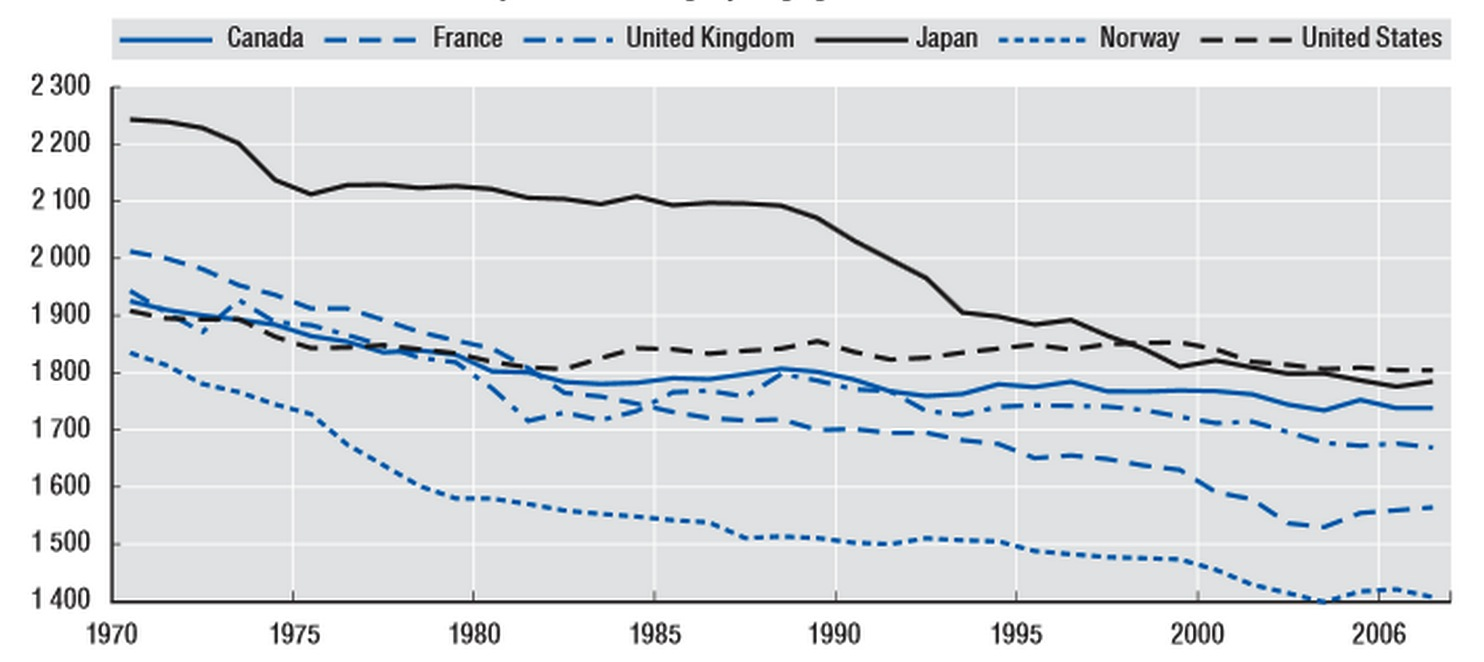
\includegraphics[width=.5\textwidth]{hoursworked}
		\cite{22}
	\end{figure}
	
	\section{Health Effects of Inactivity}
	\IEEEPARstart{I}{nactivity} carries with it major detrimental effects to human health including physical and mental afflictions. 
	The physical and mental handicaps include stress, depression, obesity and heart disease. These afflictions carry with them a reduced 
	life span and a lower quality of life.
	Obesity is an elevated topic of discussion because of the great number of detrimental effects it has on the human body. Each year there 
	are 2.8 million deaths worldwide caused by being overweight or obese. 35\% of all adults twenty years of age or older were overweight, 
	with many them being obese, according to a survey in 2008. \cite{14} Obesity and inactivity can cause cardiovascular disease, high cholesterol, 
	diabetes, different types of cancers and psychological ailments. Nearly half of all adults worldwide are affected by cardiovascular disease
	which contributes to stroke and kidney failure. There were an estimated 17.3 million deaths caused by cardiovascular disease accounting for 
	30\% of all deaths worldwide making it the number one cause of death. \cite{4}  Hypertension alone, a form of cardiovascular disease, is responsible 
	for 9.4 million deaths per year worldwide. \cite{3} Diabetes doubles the risk of death compared to peers of the same age. Diabetes will damage the 
	heart, kidney, nerves and even blood vessels. \cite{15}
	Inactivity can cause all the previous ailments, but physical activity can alleviate or even cure these effects. Physical activity increases energy 
	levels with as little as 30 minutes of exercise a day. \cite{16} This can promote many benefits at home and in the workplace such as increased 
	energy and facilitate daily tasks. Adequate physical activity can provide energy throughout the day which can increase focus on any task, physical 
	or not. \cite{17} Regular physical activity will increase cardiorespiratory and muscular fitness. \cite{3} Individuals can increase healthiness by 
	engaging in regular physical activity 150 minutes a week for adults, which is less than 30 minutes per day. \cite{18}
	In addition to the physical conditions caused by physical inactivity, it also causes many negative mental effects. These include depression, anxiety 
	and low self-esteem. Depression can cause a decrease in work performance which results in a significant decrease in employee profitability. \cite{11} 
	More than 350 million people worldwide have depression making it one of the leading causes of disabilities in the world. \cite{12} Anxiety can be beneficial 
	in small doses, but a large amount of anxiety can turn into a hindering disorder. These disorders include generalized anxiety disorder, obsessive-compulsive 
	disorder, panic disorder and post traumatic stress disorder. \cite{13}  
	With the increase in weight control that comes with physical activity, a better self-image may also be produced. Increased physical activity can cause a person 
	to look and feel more in shape. Physical activity can lead to an increase in performance and has been shown to lead to improved self-esteem. Physical activity 
	can also relieve anxiety. \cite{13} Depression will also improve with moderate levels of physical activity. \cite{17}
	As one ages, moderate aerobic and strength training activities 3-5 times a week for 30-60 minutes can improve aspects of mental health, such as improved thinking, 
	learning and judgment abilities. These activities can also help with movement, keeping joints, bones, and muscles healthy as well as slowing bone density loss. \cite{18}

\bibliographystyle{IEEEtran}

\bibliography{IEEEfull}

\end{document}